
\section{The Basic Design of the Program Repair Tool}
The program repair system can be considered as four modules: $C$ program converter, boolean program pre-processor, boolean program repair module and boolean program reverse converter.
The correlation of these four parts is shown in Figure \ref{fig:SotT}.

\begin{figure}
\centering
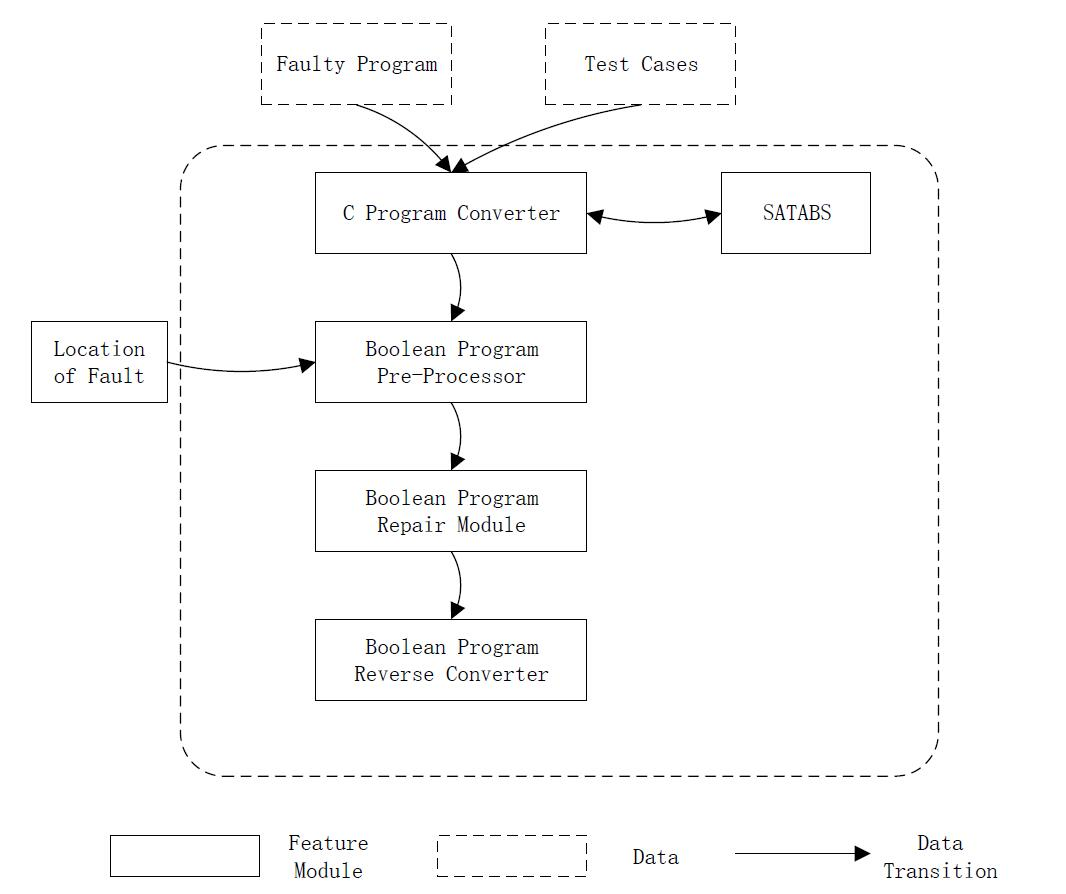
\includegraphics[width=4in,height=3.5in]{img/Fig4-1.jpg}
\caption{The Structure of the Tool}
\label{fig:SotT}
\end{figure}

\subsection{Modules of the Program Repair Tool}
We shall introduce you the details of these four components in this section.

\begin{itemize}
% C语言程序转换模块负责将C语言程序转换为布尔程序,同时对程序的变量和表达式进行谓词抽象。
\item \textbf{C program converter} is responsible for predicate abstraction and converting the given $C$ program to boolean program.
% 本模块主要调用了基于可满足性的程序抽象工具SATABS[2]来对原C语言程序进行转换。SATABS能处理C语言程序的赋值语句、控制流语句和函数调用语句等的转换,可以完成C语言程序到布尔程序的初步转换过程。
We use SATABS\cite{SATABS} to implement this module, which is capable of converting the assignment statements, control flow statements and invocation statements in $C$ program to the corresponding boolean program statements.
By doing so, this module achieves the basic conversion from $C$ program to boolean program.

\begin{itemize}
\item[-] \textbf{Input}: a faulty C program with given test cases and expected output.
\item[-] \textbf{Output}: the corresponding boolean program.
\end{itemize}

% 布尔程序预处理模块在一定程度上对C语言程序转换模块的完善。该模块对SATABS转换得出的布尔程序进行进一步的处理,
\item \textbf{Boolean program pre-processor} refines the converted boolean program to some extent. This module is capable of doing some further process on the converted boolean program,
% 去除文件中的无用信息,同时将布尔变量和其所代表的谓词以及C语言程序与布尔程序对应的位置关系提取出来。
including removing useless information, extracting the relations of boolean variables and predicates and the mappings from boolean statements to the original $C$ statements.
% 我们还在这里输入了原C语言程序出错语句的位置,使后续修复模块能够针对错误的位置进行修复。
We also input the location of the faulty $C$ statement in this process, leaving the information for further process in the following repair module.
% 本模块主要根据布尔程序的语法语义以及SATABS中C语言程序到布尔程序的转换规则对上一模块输出的文件进行分析和处理。
In summary, this module is responsible for analyzing and processing the boolean program given by last module based on the syntax and semantic of boolean programs and general conversion patterns of SATABS.

\begin{itemize}
\item[-] \textbf{Input}: a converted boolean program given by SATABS and the line number of the faulty $C$ statement in the original $C$ source file.
\item[-] \textbf{Output}: the refined boolean program and other useful related information.
\end{itemize}

% 布尔程序修复模块:对已知错误位置的布尔程序构建错误路径并计算得出正确的布尔修复。
\item \textbf{Boolean program repair module} constructs and collects all bad routes for the given boolean program and produces the appropriate boolean repair.
% 本模块可以细分为错误路径构建和修复求解两部分。
This module is actually made up of two parts: constructing bad routes and producing boolean repair.
% 错误路径构建主要是在已知错误位置的情况下,将错误语句用未知修复函数替代,并构造出所有的错误路径(见3.1.2节)。
As the location of the faulty statement is given, bad routes can be constructed by replacing the faulty statement with an unknown repairing function (\lstinline|*rep|) and listing all possible routes that lead to a wrong states (see section \ref{section:CollectingBadRoutes}).
% 修复求解则是在构建完错误路径后根据错误路径计算出修复函数的实现,即布尔修复(见3.1.3节)。
Further, the correct boolean repair will be calculated based on the set of all bad routes by taking the negation of their respective implementations (see section \ref{section:ProducingRepairingStatement}).

\begin{itemize}
\item[-] \textbf{Input}: the refined boolean program and related information.
\item[-] \textbf{Output}: boolean repair
\end{itemize}

\item \textbf{Boolean program reverse converter} converts the repaired boolean program back to $C$ language and finishes the repairing. First it will replace the boolean variables with their respective predicates
and determine the satisfiability of the converted repairing statement based on the SMT reduction described in section \ref{section:TheSatisfiabilityOfTheRepairingStatement}.
After this, several simplification rules will be applied on the converted repairing statement (section \ref{section:BooleanRepairSimplification}) to give out an effective and intuitive $C$ repairing statement.

\begin{itemize}
\item[-] \textbf{Input}: the boolean repair and the mappings produced by boolean program pre-processor.
\item[-] \textbf{Output}: the repaired $C$ program.
\end{itemize}

\end{itemize}

\subsection{Boolean Program Repair Module}
% 我们首先需要利用布尔程序修复模块找到布尔程序的正确修复。该模块又可以细分为错误路径构建和修复求解两部分。
First, boolean program repair module will be used to calculate the appropriate boolean repair. This module can be considered as two parts: constructing bad routes and calculating boolean repair.
% 在对布尔程序进行修复的时候,我们通过引入多个测试案例来确保修复结果的准确性。
Also, we improve the accuracy of this module by introducing more test cases.

% 对于一个给定的错误程序,我们需要构建出它所有可能到达错误终止状态的路径。
For a given faulty program, we need to constructs all possible routes that lead to wrong states.
% 本文以测试用例作为判断程序正确性的标准,通过assert语句来给出程序需要满足的规范,也即测试用例对应的正确输出结果。
We use test cases as the standard of a correct program in this paper, and define the specification a program should satisfy by \lstinline|assert| statements, meaning the expected output of test cases.
% 为错误程序构建错误路径时,我们会将错误语句所在的位置作为参数传入,将对应位置的语句替换为未知的修复函数,再将所有可能到达的错误状态的路径记录下来。
During the process of constructing bad routes, the location of the faulty statement will be passed as a parameter, and the faulty statement will be replaced by an unknown repairing function.
At this point, all possible bad routes will be constructed and recorded.

% 在求出了给定测试用例的所有错误路径之后,我们将对错误路径的并集取反来得到一条正确的执行路径,再进而计算该路径的具体实现。
After collecting all bad routes constructed by the given test cases, we negate the set of bad routes to produce the correct route, and further calculate the concrete implementation of this route.

\subsubsection{Multiple Test Cases Repair}
\label{section:MultipleTestCasesRepair}
% 为了确保修复结果的正确性,我们决定为一个错误程序引入多个不同的测试用例进行多次错误路径构建,从而使得到的错误路径能够完全覆盖。
More test cases means more bad routes can be constructed. In this sense, one can improve the coverage of bad routes by introducing more test cases, and by which improve the accuracy of the repairing.

% 3.1.2节中描述的代码修复方法能够根据给出的输入和正确的输出找出所有可能到达错误终止状态的错误路径。
The program repair method described in section \ref{section:CollectingBadRoutes} can find out all bad routes that lead to wrong states by given input and expected output.
% 当只给出一个测试用例时,程序的初始状态是确定的,因此在构建错误路径时所能得到的错误路径也是确定的。
For one single test case, the initial state of the program is determined, hance the bad routes can be constructed is determined.
% 不同的测试用例往往会有不同的初始状态,而在构建错误路径时,不同的初始状态到达错误状态的错误路径也是不相同的。
Different test cases can have different initial states, and different routes can be constructed to the same wrong state.
% 因此,在修复的过程中只引入一个测试用例来进行修复是不完备的。
Considering this, introducing only one test case when repairing is not completed.

% 我们针对同一个错误程序引入多个不同的测试用例,得到多个不同版本的C语言程序文件,
For one faulty program, different test cases can be introduced to generate $C$ source files of different versions.
% 再分别对它们进行错误路径构建和收集,最终再对这些结果进行分析,得出正确的修复结果。
We can still construct bad routes for each of them, and produce a more accurate repairing statement by collecting all these bad routes.
% 尽管不同版本的C语言程序转换为布尔程序后,布尔变量所代表的的谓词可能会有所不同,
$C$ source files of different versions can have different predicates and boolean variables,
% 但在找到错误路径后我们可以先对不同错误路径中的布尔变量进行合并,即对代表相同谓词的布尔变量统一命名。
but we can sum up the boolean variables in different bad routes, meaning unifying the names of boolean variables which stand for the same predicate.

\begin{theorem}
% 设引入一个测试用例对程序构建得到的错误路径集合为...,在此基础上增加测试用例对程序构建得到的错误路径集合为...,则有...。
Assume we have a set of bad routes $FP_{a}$ constructed by a test case $a$. If a new set of bad routes $FP_{b}$ can be constructed by introducing a new test case $b$,
we have $FP_{a} \subseteq FP_{b}$.
\end{theorem}

% 加入定义和定理引用
As defined in definition 3.6, the correct implementation of \lstinline|*rep| is calculated by negating the set of bad routes. If more test cases are introduces, based on theorem 4.1,
the coverage of bad routes constructed will be improved, meaning more wrong implementations of \lstinline|*rep| can be found. By doing so, we can improve the accuracy of the boolean repair.

\subsubsection{Pseudo Code}
% TO DO 插入图片并添加图片引用
% The detailed flow chart of boolean program repair module is shown in Figure 4-3, we will give out the basic implementation of this module in pseudo code in this section.

% 在对布尔程序修复构建错误路径的过程中,最重要的是模拟函数的运行过程直到终结状态通过assert语句确定该运行路径是否是错误路径
The key of constructing bad routes is to simulate the execution of the simulated function until a termination state is reached, and determine if this route is a bad route by \lstinline|assert| statement and the current evaluation.
% 模拟函数运行构建错误路径的算法基本思想是采用深度优先搜索,在进入函数时找到所有可能到达的状态,再对所有可能到达的状态进行下一步模拟进行。
All possible routes starting from a given state can be considered as a tree, while the given state being the root of the tree. The algorithm collects all possible bad routes by iterating the whole tree in a depth-first manner,
guaranteeing every state will be iterated, hence every possible route.

The pseudo code of this algorithm is shown as follows:

\begin{algorithm}
\caption{Function simulating algorithm}
\begin{algorithmic}[1]

\STATE $\textit{func} \gets \text{the function being simulated}$
\STATE $\textit{loc} \gets \text{the location of the statement being simulated}$
\STATE $\textit{eva} \gets \text{the current evaluation}$
\STATE $\textit{route} \gets \text{the current route}$
\STATE $\textit{states} \gets \text{list of all possible next states}$
\STATE $\textit{bad\_routes} \gets \text{the list of all recorded bad routes}$
\STATE

\IF {$loc == 0$}
  \IF {$\textit{loc}$ has already been simulated for $\textit{func}$}
    \RETURN existed result
  \ENDIF
\ENDIF

\STATE
\STATE push the current state to \textit{route}

\STATE
\STATE $\textit{st} \gets \textit{func}[\textit{loc}]$

\IF {$\textit{st}$ is an assignment statement}
  \IF {$\textit{st}$ is not the unknown repairing statement}
    \STATE push next state to \textit{states}
  \ELSE
    \STATE push every possible next state to \textit{states}
  \ENDIF
\ELSIF {$\textit{st}$ is an `if` statement}
  \IF {$\textit{st}$ is not the unknown repairing statement}
    \STATE push next state to \textit{states}
  \ELSE
    \STATE push every possible next state to \textit{states}
  \ENDIF
\ELSIF {$\textit{st}$ is a `goto` statement}
  \STATE push the destination state to \textit{states}
\ELSIF {$\textit{st}$ is an invocation statement}
  \STATE push every possible next state to \textit{states}
\ELSIF {$\textit{st}$ is an `assert` statement}
  \IF {$\textit{st}$ is the unknown repairing statement}
    \IF {$!check\_assert(st, eva)$}
      \STATE add \textit{route} to \textit{bad\_route}
      \RETURN the result
    \ENDIF
  \ENDIF
\ELSE
  \IF {\textit{loc} \text{is at the end of} \textit{func}}
    \RETURN the result of \textit{func}
  \ENDIF
\ENDIF

\STATE
\FORALL {state \textit{s} in \textit{states}}
  \STATE simulate \textit{s} in \textit{func}
\ENDFOR

\STATE
\IF {$loc == 0$}
  \STATE cache the result of \textit{func}
\ENDIF

\STATE
\STATE pop the current state from \textit{route}
\end{algorithmic}
\end{algorithm}

% 至此,我们已经找到了这个程序的所有错误路径,现在需要从这些错误路径中计算得到修复
So far, we collect all bad routes of a boolean program by applying the algorithm above, the next thing we need to do is to produce an appropriate boolean repair from these bad routes.
% 在3.1节中,已经证明,一个正确的修复应该不通过任意一个错误状态
In section \ref{section:BooleanProgramRepair}, we have proved that a correct boolean repair should be lead to any wrong states.
% 在每个错误路径中各取一个路径取非,再把所得路径取合取,就得到了一条正确路径
For every bad route we negate it, and conjunct all these resulting routes, and the result will be a correct path.

\begin{algorithm}
\caption{Calculates boolean repair}
\begin{algorithmic}[1]
\STATE $\textit{good\_route} \gets \text{a empty list}$
\STATE

\FORALL {\textit{route} in \textit{bad\_route}}
  \STATE negates any element of \textit{route} then put it into \textit{good\_route}
\ENDFOR

\STATE
\RETURN \textit{good\_route}

\end{algorithmic}
\end{algorithm}

% 现在计算得到了good_route,它展示了正确的*rep函数在不同的变量下的返回值,现在需要把*rep用布尔表达式表示出来。
For now, we have \lstinline|good\_route|, which stands for the correct implementation of $*rep$, represented as pairs of input and expected output of $*rep$. The last thing to do is to convert it to a readable boolean expression.
% 例如 *rep(00)=1 , *rep(01)=0 ,如果直接地表示这个布尔表达式,则应该为...
For example, we have something like $*rep(00) = 1$, $*rep(01) = 0$. Apparently, the boolean expression can be $\cap{p_{0}p_{1}} || \cap{\cap{p_{0}}p_{1}}$,
% 显然当变量多时,这种表示方式既不直观,也不方便后面的化简计算,因此我们需要更好的方式表示它。
but such representation can be complicated when the number of variables goes up, which is also difficult for further simplification.
Hence, a better representation is needed.

% 这里的实现采用了二分决策图的方法
In this case, the concept of Binary decision diagram\cite{BDD} can be introduced.
% 二分决策图是用来表示布尔函数的压缩型数据结构
The binary decision diagram (BDD) is a data structure for representing Boolean functions, which can also be considered as a compressed representation of sets or relations\cite{TfEFVUBDD,FtOVOfBDD}.
% 布尔函数可以表示为一个有根定向无环图,其中包括了决策节点和两个终端节点表示真和假,每个决策节点都被标记为一个布尔变量。一条从根节点
A Boolean function can be represented as a rooted, directed, acyclic graph, which consists of several decision nodes and terminal nodes. There are two types of terminal nodes called 0-terminal and 1-terminal.
Each decision node $N$ is labeled by boolean variable $V_{N}$ and two child nodes, representing setting the variable to $true$ or $false$.
% 一条从根节点到真值终端的路径表示该路径所代表的的变量赋值使得该布尔函数为真。
A path from the root node to a 1-terminal node means the values of variables represented by this path makes the expression to be $true$.
% 二分决策图能够消除布尔变量赋值中的冗余信息,使得其比普通的真值表表示要小很多,能够极大地压缩搜索空间
BDD can be used to eliminate duplicate information from a given boolean expression, as equivalent expressions will always produce a same BDD. Also, the representation of BDD is generally smaller than truth table,
by which the search space can be greatly reduced.

% 除了使用BDD,也可以把上面的布尔表达式展开成析取范式,并适用3.4节所证明的方法进行逻辑化简
Except for BDD, logic simplification rules described in section \ref{section:BooleanRepairSimplification} can also be applied after converting the given expression into DNF.

\subsection{Boolean Repair Reverse Converter}
% 通过布尔程序修复,我们得到了针对布尔程序的布尔修复
By applying the algorithm described in the former section, we have the boolean repair for boolean program.
% 布尔修复是由布尔变量组成的布尔表达式
Boolean repair is a boolean expression consisted of boolean variables.
% 为了得到C语言程序的修复结果,我们还需要将其转换为C语言表达式,并判断转换后的结果是否是正确且有效的。
To repair the original $C$ program, we still need to convert it to a $C$ statement and determine if the converted repairing statement is correct and effective.

% TO DO 插图,加入图片引用
% The detailed flow chart of reverse converter is shown in figure 4-4.

% 在布尔修复逆向转换模块的实现中,首先需要将布尔修复语句转换为谓词公式,在对公式的子句间和子句内进行化简
During the conversion, the first thing to do is to convert the boolean repair to its respective predicate formula.

\begin{algorithm}
\caption{Conversion of repairing clauses}
\begin{algorithmic}[1]

\STATE $\textit{clause\_str} \gets \text{the conjunctive clause to be converted}$
\STATE $\textit{vars\_map} \gets \text{mappings from boolean variables to predicates}$
\STATE $\textit{predicates} \gets \text{the list of converted predicates}$
\STATE

\STATE $\textit{vars\_str} \gets \text{split}(\textit{clause\_str}, \text{"\&"})$
\FORALL {\textit{var\_str} in \textit{vars\_str}}
  \STATE $\textit{isNeg} \gets \text{if the current variable is a negation}$
  \IF {\textit{var\_str}[0] == \textit{'!'}}
    \STATE $\textit{isNeg} \gets true$
    \STATE $\textit{var\_str} \gets \textit{var\_str}.\text{substr}(1)$
  \ELSE
    \STATE $\textit{isNeg} \gets false$
  \ENDIF
  \STATE
  \STATE $\textit{predicate} \gets \textit{vars\_map}.map(\textit{var\_str})$
  \IF {\textit{isNeg}}
    \STATE $\textit{predicate} \gets \textit{predicate}.\text{negate}()$
  \ENDIF
  \STATE \textit{predicates}.push(\textit{predicate})
\ENDFOR
\STATE
\RETURN \textit{predicates}

\end{algorithmic}
\end{algorithm}

\begin{algorithm}
\caption{Conversion of repairing expression}
\begin{algorithmic}[1]

\STATE $\textit{expr\_str} \gets \text{the disjunctive expression to be converted}$
\STATE $\textit{clauses} \gets \text{the list of converted clauses}$
\STATE

\STATE $\textit{clauses\_str} \gets \text{split}(\textit{expr\_str}, "\mid")$

\FORALL {\textit{clause\_str} in \textit{clauses\_str}}
  \STATE $\textit{clause} \gets \text{clause\_conversion}(\textit{clause\_str})$
  \IF {\textit{clause} is always \textit{true}}
    \RETURN always \textit{true}
  \ENDIF
  \STATE \textit{clauses}.push(\textit{clause})
\ENDFOR

\end{algorithmic}
\end{algorithm}

As the repairing statement generated by the tool will always be in DNF, simplification can be applied to produce a more readable statement.
Several effective simplification rules are described in section \ref{section:BooleanRepairSimplification}, while applying BDD for simplification is also acceptable.

\subsection{Complexities of Algorithms}
% 前文给出了布尔程序修复逆向转换工具的具体实现及算法,该工具可以看作一个整体的完善的修复系统。我们将在这里给出工具每个模块实现算法的时间复杂度的分析。
In the former sections, we described the basic implementation of the program repair tool. In this section, the time complexity of different modules will be analyzed.

% C程序转换模块调用了外部的SATABS程序来将C程序转换为布尔程序,因此这部分的算法复杂度不作考虑。
The $C$ program converter is implemented by using SATABS to convert a $C$ program to boolean program, hence the complexity of this module will not be considered.

% 布尔程序预处理模块算法的时间复杂度是常数级别的
The algorithm used to implement boolean program pre-processor is constant time.
% 该模块提取除了布尔程序的变量个数以及C程序语句和布尔程序语句的映射关系
This module is responsible for extracting the information of boolean variables and the mappings from $C$ statements to boolean statements.
% 具体实现时利用了SATABS对C程序转换为布尔程序过程中产生的信息,只需要对C程序和布尔程序各查找常数次
Such intermediate information will be generated when SATABS is converting the $C$ program, constant number of searches on both source files is all we need.
% 设转换前的C程序行数为LoC,转换后的布尔程序的行数为LoBP,则这部分算法的复杂度为...
If we have to consider the length of source files, let's assume the number of lines in the original $C$ program is $LoC$ and the converted boolean program is $LoBP$,
then the complexity of this algorithm should be $O(LoC + LoBP)$.

% 布尔程序修复模块部分的算法复杂度是整个工具的瓶颈
The boolean program repair module is actually the bottleneck of the whole system.
% 设布尔程序的变量个数为.., 则布尔程序运行过程中,变量的赋值空间为...,因此总的可能的运行路径数为...在程序运行过程中产生的不同的状态数为...
Assume the number of boolean variables is $V$, then the number of evaluations could be $X = O(2^{V})$, which means the number of possible routes is $O(2^{X})$,
and the number of distinct states is $O(LoBP * X)$.
In this sense, the number of routes grows exponentially as the number of boolean variables grows, which also grows exponentially as the number of variables in the original $C$ program grows. It would appear to be the major bottleneck of the whole system. The complexity of this module is $O(LoBP * X + 2^{X})$.

% 在整个布尔程序逆向转换工具中,布尔程序修复算法是整个系统的瓶颈所在,因此需要对其进行优化。
As the bottleneck of the whole system, optimization can be applied on this module.
% 在本文的实现中,采用了减少模拟运行过程中需要考虑的变量数来进行优化,即减少V的大小
In our implementation, we use different ways to reduce the number of variables need to be considered during the simulation, meaning reducing $V$.
% 由于 X = 2^V,V的减少会对算法的复杂度进行极大地优化
As $X = 2^{V}$, no doubt the reduction on $V$ can greatly facilitate the performance of the algorithm.
% 这种优化方法是可行且正确的,因为在每一步的运算过程中,大部分变量都为临时变量或与当前运算不相关的变量,
Such optimization is actually effective, as for each statement, most accessible variables are of temporary use or irrelevant to the simulating statement.
% 因此可以只将当前的非临时且与运算有关的变量提取出来,只考虑这些变量在路径中的状态变迁。
In this case, we only consider the state transitions of those variables which is not temporary and is relevant to the current statement during the simulation.
% 这将使得布尔程序修复部分的运行时间大幅减少并在可接受范围内
By doing so, the time cost needed for boolean program repair is greatly reduced and become more acceptable.

% 在布尔修复逆向转换模块,最关键的工作是将一个布尔程序语句转换成C程序语句并根据语义进行化简。
Boolean repair reverse converter is responsible for converting boolean statement back to respective $C$ statement and apply simplification based on its semantic.
% 在整个转换及化简的过程中,修复表达式始终保持为析取范式。
Note that the repairing expression will maintain to be in DNF in the whole process.
% 设析取范式的修复子式个数为N,每个修复子式中最大的谓词个数为M。
Assume the number of clauses in the DNF expression is $N$, and the maximum number of predicates in each clause is $M$.
% 对一个修复子式执行子句内化简时,将谓词按照它们的语义进行排序,并合并了语义可化简的谓词。
During the process of inner-clause simplification, predicates will be sorted based on their semantics, and those predicates with similar semantics will be combined as one.
% 谓词的排序可以采用快速排序,算法的复杂度为O(MlogM),而排序后可合并的谓词只会相邻出现,因此合并的算法复杂度为O(M)。
The sort of predicates can be implemented by quick sort, whose complexity is $O(M\log{M})$. After the predicates are in order, those predicates with combinable semantics will only appear consecutively,
so the complexity of finding combinable predicates is $O(M)$.
% 由此,对所有修复子式执行子句内化简的算法复杂度为O(NMlogM)。
In this sense, the complexity of inner-clause simplification for all clauses is $O(NM\log{M})$.
% 执行子句间化简时,需要枚举两个修复子式,并检查两个修复子式中每个谓词的含义是相同还是相反,因此算法的时间复杂度为O(N^2M^2)
Each pair of clauses will checked for whether their predicates have same or exactly opposite meanings in the process of inter-clause simplification, hence the complexity is $O(N^{2}M^{M})$.
% 执行子句外化简时,需要检查每个子句的可满足性,而检查子句的可满足性属于SMT问题。
As for outer-clause simplification, the satisfiability of each clause will be examined, which can be reduced to SMT problem.
% SMT问题是个NP完全问题,不存在多项式时间算法,因此最坏情况下的时间复杂度为O(2^M)。
SMT program is an NP-complete problem, which can be verified in polynomial time, so the complexity of outer-clause simplification will be $O(2^{M})$ in the worst case.
% 由于先执行了子句内化简,子句中的谓词数量减少,能有效地降低时间复杂度。
But outer-clause simplification actually preforms after inner-clause simplification, which can reduce the number of predicates in clauses, hence reduce the time cost needed for outer-clause simplification.
% 因此,布尔修复逆向转换的总体复杂度为...
In summary, the time complexity of boolean repair reverse conversion is $O(NM\log{M} + N2^{M} + N^{2}M^{2})$.
